\documentclass[11pt, a4paper]{article}
\usepackage[utf8]{inputenc}
\usepackage{minted}
\usepackage{hyperref}
\usepackage{graphicx}
\usepackage{amsmath}
\usepackage{subcaption}
\graphicspath{{./images/}}

\begin{document}
\title{Extended Kalman Filters}
\author{Samuel Navarro}
\date{\today}
\maketitle
\tableofcontents{}


Is called extended in a sense that it will be capable of handling more complex motion and measurement models. 

\begin{figure}[htpb!]
	\centering
	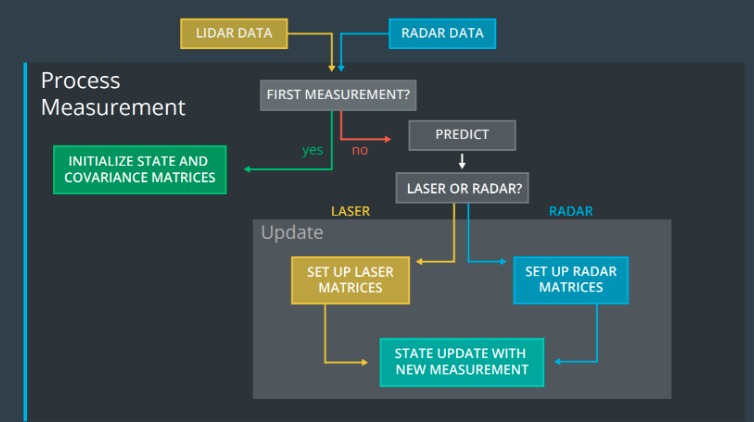
\includegraphics[width=0.8\linewidth]{kalman_filter_algorithm}
	\caption{Kalman Filter Algorithm}
	\label{fig:kalman_filter_algorithm}
\end{figure}


You have two sensors (Lidar and Radar) and the information provided by this sensors is used to estimate the state of a moving pedestrian and this state is represented by a 2D position and 2D velocity (Figure~\ref{fig:states}.) Each time we receive information by a given sensor, the estimation function is triggered. 

\begin{figure}[htpb!]
	\centering
	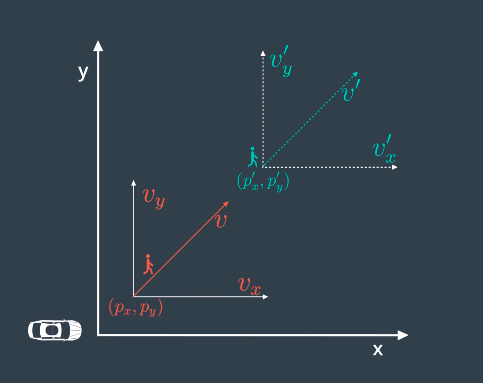
\includegraphics[width=0.8\linewidth]{states}
	\caption{State}
	\label{fig:states}
\end{figure}




The \textbf{Kalman Filter} algorithm will go through the following steps:
\begin{itemize}
	\item \textbf{first measurement} - the filter will receive initial measurements of the bicycle's positions relative to the car. The measurements will come from a radar or lidar sensor. 
	\item \textbf{Initialize state and covariance matrices} - the filter will initialize the bicycle's positions based on the first measurement.
	\item The car will receive another sensor measurement after a time period $\Delta t$.
	\item \textbf{predict} - the algorithm will predict where the bicycle will be after time $\Delta t$. We will assume the velocity is constant, hence, the bicycle will have moved velocity * $\Delta t$.
	\item \textbf{update}: The filter compares the "predicted" location with what the sensor measurement says. The predicted location and the measured location are combined to give an update location. The Kalman filter will put more weight on either the predicted location or the measured location depending on the uncertainty of each value. 
	\item The car will receive another sensor measurement after a time period $\Delta t$. The algorithm then does another \textbf{predict} and \textbf{update} step.
\end{itemize}






At its core, the Kalman filter is a two-step estimation problem represented in Figure~\ref{fig:two-step}.

\begin{figure}[htpb!]
	\centering
	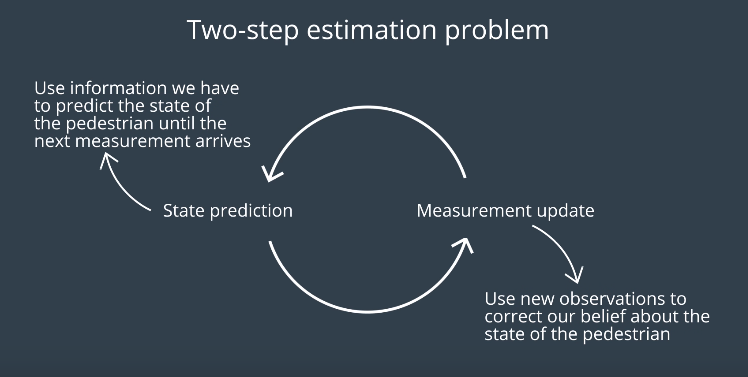
\includegraphics[width=0.8\linewidth]{two-step}
	\caption{Two-step estimation problem}
	\label{fig:two-step}
\end{figure}


But what happens when there are two sensors that observe the same pedestrian? This is represented in Figure~\ref{fig:2-sensors}

\begin{figure}[htpb!]
	\centering
	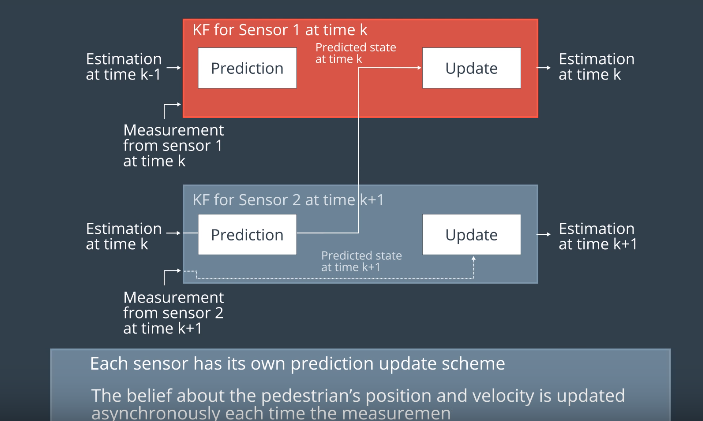
\includegraphics[width=0.8\linewidth]{2-sensors}
	\caption{2 Sensors}
	\label{fig:2-sensors}
\end{figure}



The Figure~\ref{fig:example_flow} is an example flow to see how this works:


\begin{figure}[htpb!]
	\centering
	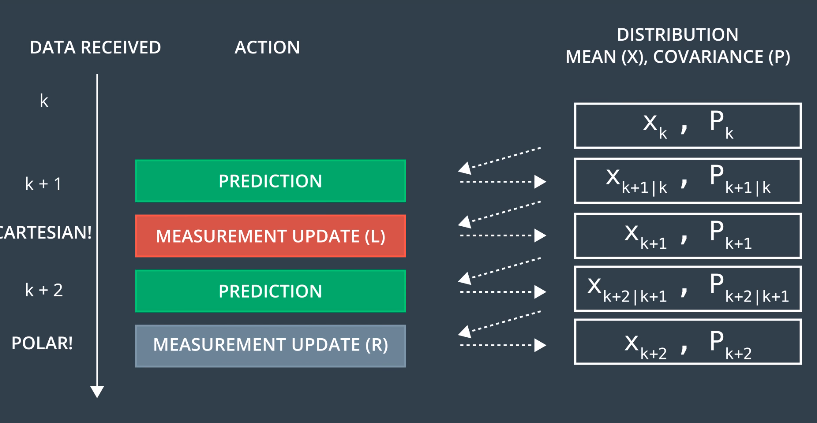
\includegraphics[width=0.8\linewidth]{example_flow}
	\caption{Flow example}
	\label{fig:example_flow}
\end{figure}







\textbf{Definition of Variables}
\begin{itemize}
	\item x is the mean state vector. For an extended Kalman filter, the mean state vector contains information about the object's position and velocity that you are tracking. It is called the "mean" state vector because position and velocity are represented by a gaussian distribution with mean x.
	\item P is the state covariance matrix, which contains information about the uncertainty of the object's position and velocity. You can think of it as containing standard deviations.
	\item k represents time steps. So $x_k$ refers to the object's position and velocity vector at time k.
	\item The notation $k+1|k$ refers to the prediction step. At time $k+1$, you receive a sensor measurement. Before taking into account the sensor measurement to update your belief about the object's position and velocity, you predict where you think the object will be at time $k+1$. You can predict the position of the object at $k+1$ based on its position and velocity at time $k$. Hence $x_{k+1|k}$  means that you have predicted where the object will be at k+1 but have not yet taken the sensor measurement into account.
	\item $x_{k+1}$ means that you have now predicted where the object will be at time k+1 and then used the sensor measurement to update the object's position and velocity.

\end{itemize}




What should a \textbf{Kalman Filter} do if both the radar and laser measurements arrive at the same time \textbf{$k+3$}?

R: Predict the state to $k+3$ then use either one of the sensors to update. Then predict the state to $k+3$ again and update with the other sensor measurement.


Because we have already run a prediction-update iteration with the first sensor at time $k+3$, the output of the second prediction at time $k+3$ will actually be identical to the output from the update step with the first sensor. So, in theory, you could skip the second prediction step and just run a prediction, update, update iteration.

This is represented in Figure~\ref{fig:2-sensors-quiz}

\begin{figure}[htpb!]
	\centering
	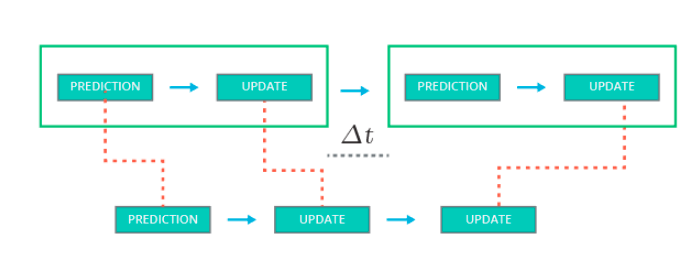
\includegraphics[width=0.8\linewidth]{2-sensors-quiz}
	\caption{Prediction-Update-Update}
	\label{fig:2-sensors-quiz}
\end{figure}


The \textit{state transition function} model how the state has changed from time $k-1$ to time $k$.


\begin{figure}[htpb!]
	\centering
	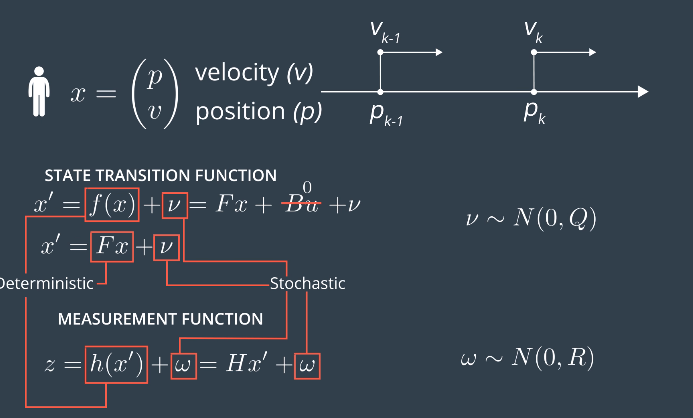
\includegraphics[width=0.8\linewidth]{state_and_measurement_func}
	\caption{State and Measurement Function}
	\label{fig:state_and_measurement_func}
\end{figure}





\begin{figure}[htpb!]
	\centering
	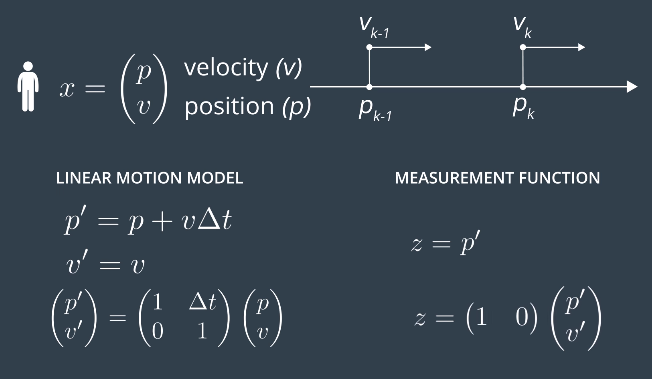
\includegraphics[width=0.8\linewidth]{linear_motion_measurement}
	\caption{Linear Motion Measurement}
	\label{fig:linear_motion_measurement}
\end{figure}



\begin{figure}[htpb!]
	\centering
	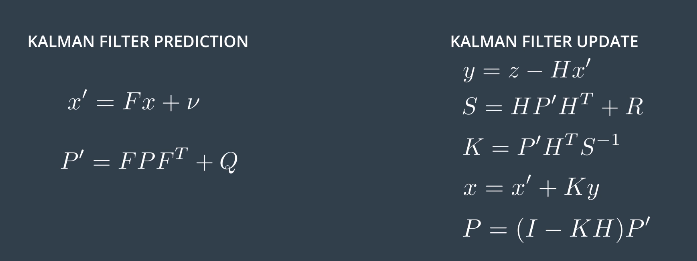
\includegraphics[width=0.8\linewidth]{KF_update_predict}
	\caption{Kalman Filter Update and Predict}
	\label{fig:KF_update_predict}
\end{figure}


\textbf{Kalman Filter Intuition} \\

\textbf{Prediction} \\


Let's say we know an object's current position and velocity , which we keep in the x variable. Now one second has passed. We can predict where the object will be one second later because we knew the object position and velocity one second ago; we'll just assume the object kept going at the same velocity.

The $x' = Fx + \nu$ equation does these prediction calculation for us.

But maybe the object didn't maintain the exact same velocity. Maybe the object changed direction, accelerated or decelerated. So when we predict the position one second later, out uncertainty increases. $P' = FPF^T + Q$ represents this increase in uncertainty.

Process noise refers to the uncertainty in the prediction step. We assume the object travels at a constant velocity, but in reality, the object might accelerate or decelerate. The notation $\nu 
\sim N(0,Q)$ defines the process noise as a gaussian distribution with mean zero and covariance Q.

\textbf{Update} \\

Now we get some sensor information that tells where the object is relative to the car. First we compare where we think we are with what the sensor data tells us $y = z - Hx'$


The $K$ matrix, often called the \textbf{Kalman Filter} gain, combines the uncertainty of where we think we are $P'$ with the uncertainty of our sensor measurement $R$. 

\begin{itemize}
	\item If our sensor measurements are very uncertain (R is high relative to $P'$) then the Kalman filter will give more weight to where we think we are: $x'$. 
	\item If where we think we are is uncertain ($P'$ is high relative to $R$), the Kalman filter will put more weight on the sensor measurement: z.

\end{itemize}

Measurement noise refers to uncertainty in sensor measurements. The notation $\omega \sim N(0,R)$ defines the measurement noise as a gaussian distribution with mean zero and covariance $R$. Measurement noise comes form uncertainty in sensor measurements.


\textbf{A Note about the State Transition Function: Bu} \\

If you go back to the video, you'll notice that the state transition function was first given as $x' = Fx + Bu + \nu$.

$B$ is a matrix called the control input matrix and $u$ is the control vector.


As an example, let's say we were tracking a car and we knew for certain how much the car's motor was going to accelerate or decelerate over time; in other words, we had an equation to model the exact amount of acceleration at any given moment. $Bu$ would represent the updated position of the car due to the internal force of the motor. We would use $\nu$ to represent any random noise that we could not precisely predict like if the car slipped on the road or a strong wind moved the car.

For the Kalman filter lessons, we will assume that there is no way to measure or know the exact acceleration of a tracked object. For example, if we were in an autonomous vehicle tracking a bicycle, pedestrian or another car, we would not be able to model the internal forces of the other object; hence, we do not know for certain what the other object's acceleration is. Instead, we will set $Bu = 0$ and represent acceleration as a random noise with mean $\nu$.



In the Lesson map~\ref{fig:lesson_map} we see that we need the process Covariance matrix to model the stochastic part of the state transition model. 
\begin{figure}[htpb!]
	\centering
	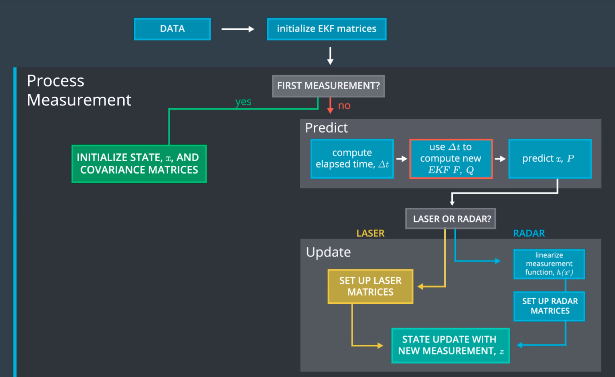
\includegraphics[width=0.8\linewidth]{lesson_map}
	\caption{Lesson Map}
	\label{fig:lesson_map}
\end{figure}



In Figure~\ref{fig:kinematic_eq} we can see how acceleration is expressed by the \textbf{kinematic equations} and then we use that information to derive the process covariance matrix. ($Q$).
\begin{figure}[htpb!]
	\centering
	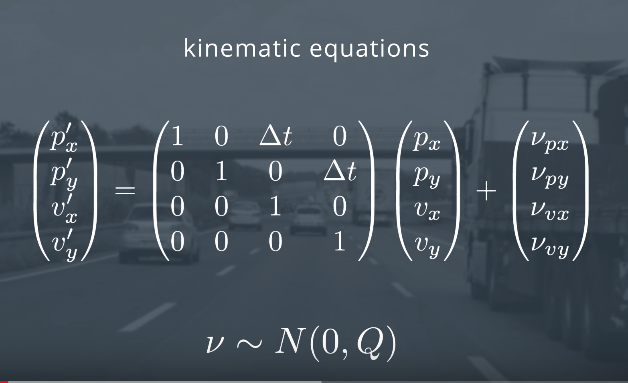
\includegraphics[width=0.8\linewidth]{kinematic_eq}
	\caption{Kinematic Equations}
	\label{fig:kinematic_eq}
\end{figure}


\section{Process Covariance Matrix}%
\label{sec:process_covariance_matrix}


As a reminder, here are the state covariance matrix update equation and the equation for Q.


$ P = FPF^T + Q $

\[
Q=\left(\begin{array}{cccc}{\frac{\Delta t^{4}}{4} \sigma_{a x}^{2}} & {0} & {\frac{\Delta t^{3}}{2} \sigma_{a x}^{2}} & {0} \\ {0} & {\frac{\Delta t^{4}}{4} \sigma_{a y}^{2}} & {0} & {\frac{\Delta t^{3}}{2} \sigma_{a y}^{2}} \\ {\frac{\Delta t^{3}}{2} \sigma_{a x}^{2}} & {0} & {\Delta t^{2} \sigma_{a x}^{2}} & {0} \\ {0} & {\frac{\Delta t^{3}}{2} \sigma_{a y}^{2}} & {0} & {\Delta t^{2} \sigma_{a y}^{2}}\end{array}\right)
.\] 


\[
	\left\{\begin{array}{l}{p_{x}^{\prime}=p_{x}+v_{x} \Delta t+\frac{a_{x} \Delta t^{2}}{2}} \\ 
	{p_{y}^{\prime}=p_{y}+v_{y} \Delta t+\frac{a_{y} \Delta t^{2}}{2}} \\ {v_{x}^{\prime}=v_{x}+a_{x} \Delta t} \\ {v_{y}^{\prime}=v_{y}+a_{y} \Delta t}\end{array}\right.
.\] 




Since the acceleration is unknown we can add it to the noise component, and this rnadom noise would be expressed analytically as the last terms in the equation derived above. So, we have a random acceleration vector $\nu$ in this form:

\[
\nu=\left(\begin{array}{c}{\nu_{p x}} \\ {\nu_{p y}} \\ {\nu_{v x}} \\ {\nu_{v y}}\end{array}\right)=\left(\begin{array}{c}{\frac{a_{x} \Delta t^{2}}{2}} \\ {\frac{a_{y} \Delta t^{2}}{2}} \\ {a_{x} \Delta t} \\ {a_{y} \Delta t}\end{array}\right)
.\] 

Which is described by a zero mean and a covariance matrix Q, so $\nu \sim N(0,Q)$


The $\nu$ vector can be decomposed into two components:

\[
\nu=\left(\begin{array}{c}{\frac{a_{x} \Delta t^{2}}{2}} \\ {\frac{a_{y} \Delta t^{2}}{2}} \\ {a_{x} \Delta t} \\ {a_{y} \Delta t}\end{array}\right)=\left(\begin{array}{cc}{\frac{\Delta t^{2}}{2}} & {0} \\ {0} & {\frac{\Delta t^{2}}{2}} \\ {\Delta t} & {0} \\ {0} & {\Delta t}\end{array}\right)\left(\begin{array}{l}{a_{x}} \\ {a_{y}}\end{array}\right)=G a
.\] 



$\Delta t$ is computed at each Kalman Filter step and the acceleration is a random vector with zero mean and standard deviations $\sigma_{ax}$ and $\sigma_{ay}$.


We now define Q as:


\begin{equation} \label{process_cov_matrix}
\begin{split}
	Q & = E[\nu \nu^T] - E[\nu]E[\nu]^T \\
	  & = E[\nu \nu^T] \\
	  & = E[G a a^T G^T] \\
	  & = GE[aa^T]G^T \\
	  & = G\left(\begin{array}{cc}{\sigma_{a x}^{2}} & {\sigma_{a x y}} \\ {\sigma_{a x y}} & {\sigma_{a y}^{2}}\end{array}\right) G^{T} \\
	  & = GQ_{\nu}G^T
\end{split}	
\end{equation}

With:
\[
G = \left(\begin{array}{cc}{\frac{\Delta t^{2}}{2}} & {0} \\ {0} & {\frac{\Delta t^{2}}{2}} \\ {\Delta t} & {0} \\ {0} & {\Delta t}\end{array}\right)
.\] 

Where $Q_{\nu}$:


\[
Q_{\nu}=\left(\begin{array}{cc}{\sigma_{a x}^{2}} & {\sigma_{a x y}} \\ {\sigma_{a x y}} & {\sigma_{a y}^{2}}\end{array}\right)=\left(\begin{array}{cc}{\sigma_{a x}^{2}} & {0} \\ {0} & {\sigma_{a y}^{2}}\end{array}\right)
.\] 


This give us:

\[
Q=G Q_{\nu} G^{T}=\left(\begin{array}{cccc}{\frac{\Delta t^{4}}{4} \sigma_{a x}^{2}} & {0} & {\frac{\Delta t^{3}}{2} \sigma_{a x}^{2}} & {0} \\ 
{0} & {\frac{\Delta t^{4}}{4} \sigma_{a y}^{2}} & {0} & {\frac{\Delta t^{2}}{2} \sigma_{a y}^{2}} \\ 
{\frac{\Delta t^{3}}{2} \sigma_{a x}^{2}} & {0} & {\Delta t^{2} \sigma_{a x}^{2}} & {0} \\ 
{0} & {\frac{\Delta t^{3}}{2} \sigma_{a y}^{2}} & {0} & {\Delta t^{2} \sigma_{a y}^{2}}\end{array}\right)
.\] 


\section{Laser Measurements}%
\label{sec:laser_measurements}



The measurement vector is $z$.
Measurement matrix is $H$.
Covariance matrix, $R$.


\begin{figure}[htpb!]
	\centering
	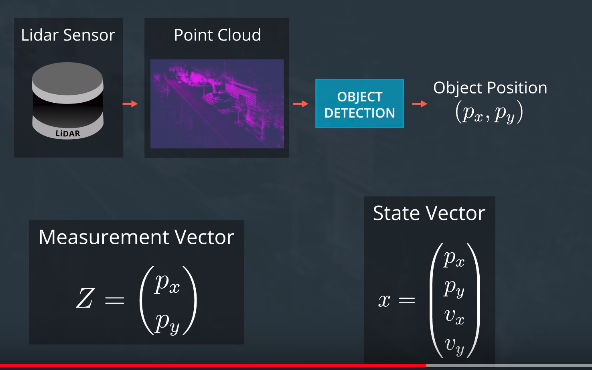
\includegraphics[width=0.8\linewidth]{lidar_p1}
	\caption{Lidar Measurement P 1}
	\label{fig:lidar_p1}
\end{figure}


\begin{itemize}
	\item z is the measurement vector. For a lidar sensor, the $z$ vector contains the position x and position y measurements.
	\item $H$ is the matrix that projects your belief about the object's current state into the measurement space of the sensor. For lidar, this is a fancy way of saying that we discard velocity information from the state variable since the lidar sensor only measures position: The state vector $x$ contains information about $[p_x, p_y, v_x, v_y]$ whereas the $z$ vector will only contain $[px, py]$. Multiplying $Hx$ allows us to compare x, our belief, with z, the sensor measurement.
	\item What does the prime notation in the $x$ vector represent? The prime notation like $p_x'$ means you have already done the prediction step but have not done the measurement step yet. In other words, the object was at $p_x$. After time $\Delta{t}$, you calculate where you believe the object will be based on the motion model and get $p_x'$ .
\end{itemize}


\textbf{Quiz}\\

Find the right $H$ matrix to project from a 4D state to a 2D observation space, as follows:


\[
\left(\begin{array}{c}{p_{x}} \\ {p_{y}}\end{array}\right)=H\left(\begin{array}{c}{p_{x}^{\prime}} \\ {p_{y}^{\prime}} \\ {v_{x}^{\prime}} \\ {v_{y}^{\prime}}\end{array}\right)
.\] 

with 

\[
H=\left(\begin{array}{llll}{1} & {0} & {0} & {0} \\ {0} & {1} & {0} & {0}\end{array}\right)
.\] 


Now, the \textbf{Measurement Noise Covariance Matrix} we have:

\[
R=E\left[\omega \omega^{T}\right]=\left(\begin{array}{cc}{\sigma_{p x}^{2}} & {0} \\ {0} & {\sigma_{p y}^{2}}\end{array}\right)
.\] 

Generally, the parameters for the random noise measurement matrix will be provided by the sensor manufacturer. For the extended Kalman filter project, we have provided $R$ matrices values for both the radar sensor and the lidar sensor. 


Because we have 0 in the off-diagonal, we know that the noise processes are uncorrelated.




\textbf{More Info on Timestamps} \\




\begin{figure}[htpb!]
	\centering
	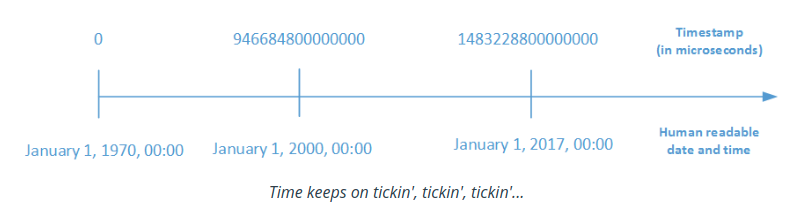
\includegraphics[width=0.8\linewidth]{timestamps}
	\caption{Timestamps}
	\label{fig:Timestamps}
\end{figure}


We can use the timestamps values to compute the elapsed time between two consecutive observations as:

\texttt{float delta\_t = (timestamp(k+1) - timestamp(k) ) / 1000000.0 } 


\begin{figure}[h!]
 
\begin{subfigure}{0.5\textwidth}
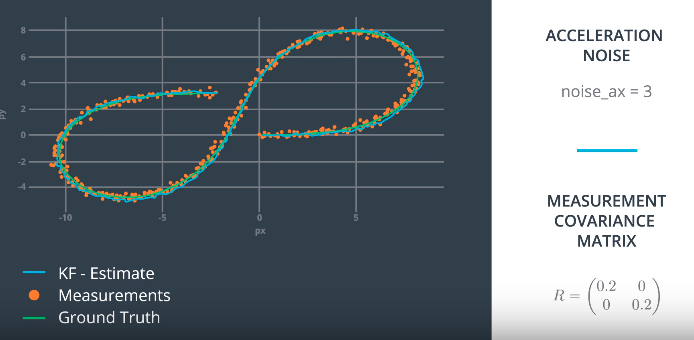
\includegraphics[width=0.9\linewidth, height=5cm]{KF_estimate_0} 
\caption{Kalman Filter Estimate}
\label{fig:subim1}
\end{subfigure}
\begin{subfigure}{0.5\textwidth}
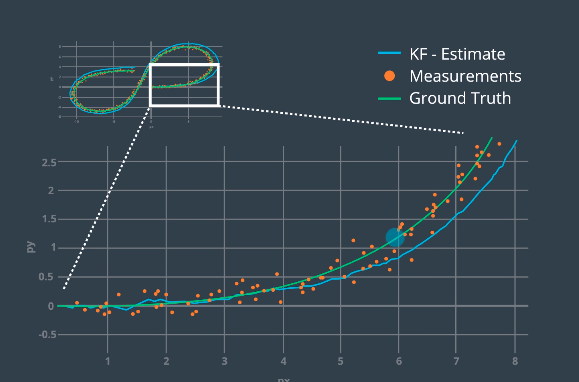
\includegraphics[width=0.9\linewidth, height=5cm]{KF_estimate}
\caption{Caption 2}
\label{fig:subim2}
\end{subfigure}
 
\caption{Kalman Filter Estimate Process}
\label{fig:image2}
\end{figure}



We see that if we change the \textbf{Measurement Covariance matrix} to higher values, the estimations is not going to go well in the curved parts. 

So, we need to check the measurement or the process noises. 

\section{Radar Measurements}%
\label{sec:radar_measurements}



We want to combine both sensors:

\begin{figure}[htpb!]
	\centering
	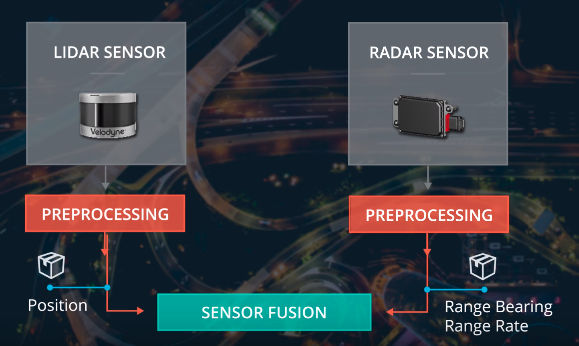
\includegraphics[width=0.8\linewidth]{sensor_fusion}
	\caption{Sensor Fusion}
	\label{fig:sensor_fusion}
\end{figure}


\begin{figure}[htpb!]
	\centering
	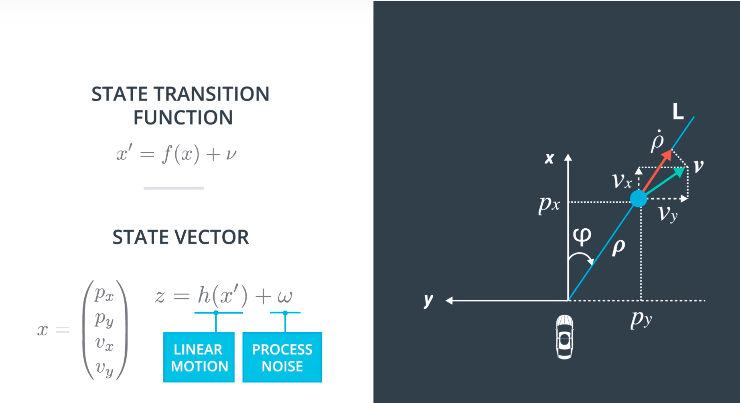
\includegraphics[width=0.8\linewidth]{radar_measurements}
	\caption{Radar measurements}
	\label{fig:radar_measurements}
\end{figure}



Where:
\begin{itemize}
	\item Range: $\rho$ is radial distance from origin.
	\item Bearing. $\varphi$ is the angle between $\rho$ and $x$
	\item Radial Velocity: $\dot{\rho}$ is the change of $\rho$
\end{itemize}



Now, considering that the three measurement vector components are not cross-correlated, the radar measurement covariance matrix becomes:



\begin{figure}[htpb!]
	\centering
	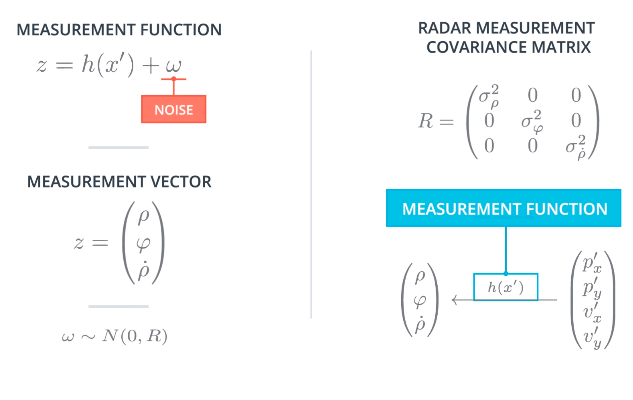
\includegraphics[width=0.8\linewidth]{measurement_radar}
	\caption{Measurement Radar}
	\label{fig:measurement_radar}
\end{figure}




\textbf{H versus h(x)} \\

The $H$ matrix from the lidar lesson and $h(x)$ equations from the radar lesson are actually accomplishing the same thing; they are both needed to solve $y = z - Hx'$ in the update step.

But for radar, there's no $H$ matrix that will map the state vector $x$ into polar coordinates; instead, you need to calculate the mapping manually to convert from cartesian coordinates to polar coordinates.

Here is the $h$ function that specifies how the predicted position and speed get mapped to the polar coordinates of range, bearing and range rate.


\[
	h\left(x^{\prime}\right)=\left(\begin{array}{c}{\rho} \\ {\varphi} \\ {\dot{\rho}}\end{array}\right)= \left(\begin{array}{c}{\sqrt{p_{x}^{\prime 2}+p^{\prime2}_{y}}} \\ 
	{\operatorname{arctan}\left(p_{y}^{\prime} / p_{x}^{\prime}\right)} \\ 
{\frac{p_{x}^{\prime} v_{x}^{\prime}+p_{y} v_{y}^{\prime}}{\sqrt{p_{x}^{\prime2}+p_{y}^{\prime2}}}}\end{array}\right)
.\] 


Hence for radar $y = z - Hx'$ becomes $y = z - h(x')$.



\textbf{Definition of Radar Variables} \\

\begin{itemize}
	\item The range, $\rho$ is the distance to the pedestrian. The range is basically the magnitude of the position vector $\rho$ which can be defined as $\rho = \sqrt{p_{x}^2 + p_{y}^2}$
	\item $\varphi \operatorname{atan} \frac{p_y}{p_x}$. Note that $\varphi$ is referenced counter-clockwise from the x-axis, so the $\varphi$ from the video clip above in that situation would actually be negative.
	\item The range rate, $\dot{\rho}$ is the projection of the velocity, $\nu$, onto the line, $L$.
\end{itemize}




\textbf{Quiz} \\
What happens if we have a nonlinear measurement function, h(x). Can we apply the \textbf{Kalman Filter} equations to update the predicted state, X, with new measurements, z?
It turns out that applying a nonlinear function to a Gaussian distribution removes its "Gaussianness". 

\begin{figure}[htpb!]
	\centering
	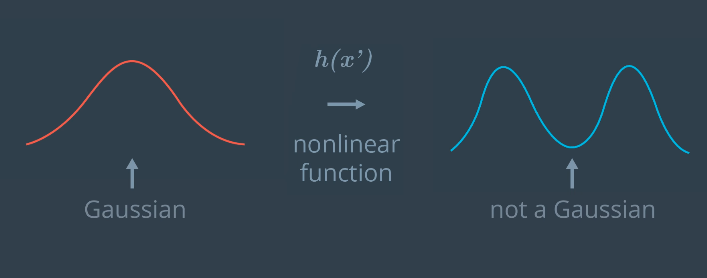
\includegraphics[width=0.8\linewidth]{not_Gaussian}
	\caption{Non linear function to a Gaussian}
	\label{fig:not_Gaussian}
\end{figure}



\begin{figure}[htpb!]
	\centering
	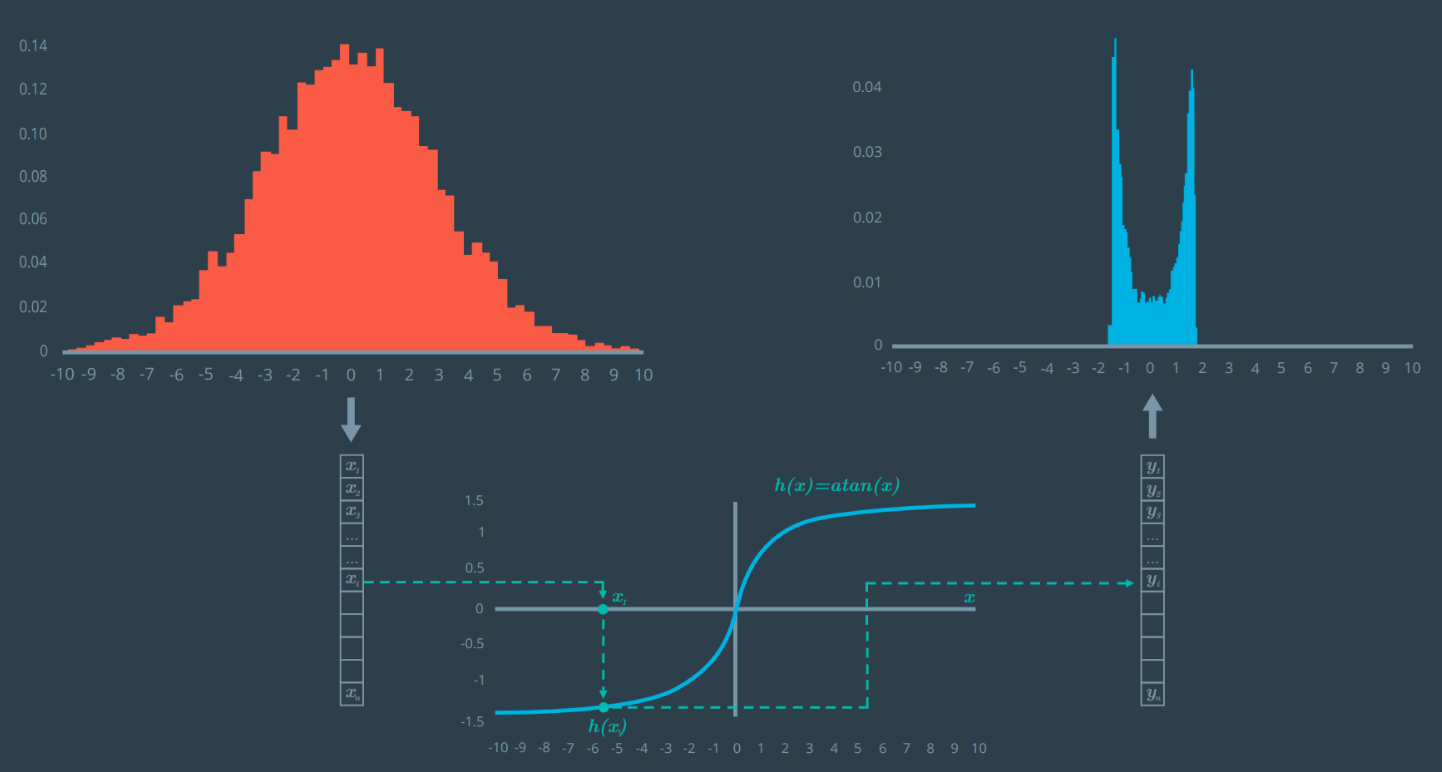
\includegraphics[width=0.8\linewidth]{non_linear_to_gaussian}
	\caption{Non-Linear to Gaussian}
	\label{fig:non_linear_to_gaussian}
\end{figure}




We can see in Figure~\ref{fig:non_linear_to_gaussian} that after applying a non-linear function, the result is not Gaussian, so, we will try to approximate this with a Taylor approximation. That's why this is called \textbf{Extended Kalman Filter}. 




\begin{figure}[htpb!]
	\centering
	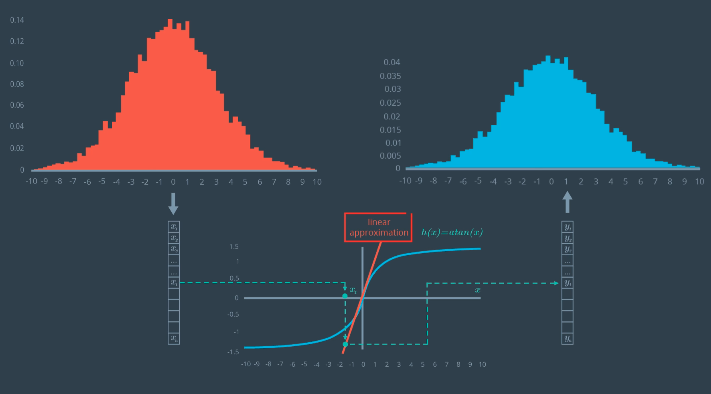
\includegraphics[width=0.8\linewidth]{linear_approx}
	\caption{Linear approximation to Gaussian returns Gaussian}
	\label{fig:linaer_approx}
\end{figure}

The \textbf{Extended Kalman Filter} uses \textbf{First Order Taylor Expansion}

\[
	h(x) \approx h(\mu) + \frac{\partial h(\mu)}{\partial x} (x - \mu)
.\] 




\textbf{Multivariate Taylor Series} \\

Recall from the \textit{Radar Measurements} lecture that the h function is composed fo three equations that show how the predicted state, $x' = (p'_x, p'_y, \nu'_x, \nu'_y)^T$, is mapped into the measurement space, $z = (\rho, \varphi, \dot{\rho})^T$



\[
	h\left(x^{\prime}\right)=\left(\begin{array}{c}{\rho} \\ {\varphi} \\ {\dot{\rho}}\end{array}\right)= \left(\begin{array}{c}{\sqrt{p_{x}^{\prime 2}+p^{\prime2}_{y}}} \\ 
	{\operatorname{arctan}\left(p_{y}^{\prime} / p_{x}^{\prime}\right)} \\ 
{\frac{p_{x}^{\prime} v_{x}^{\prime}+p_{y} v_{y}^{\prime}}{\sqrt{p_{x}^{\prime2}+p_{y}^{\prime2}}}}\end{array}\right)
.\] 





These are multi-dimensional equations so we need to use a multi-dimensional Taylor series expansion. Here's the general formula for the multi-dimensional Taylor series expansion:


\[
T(x)=f(a)+(x-a)^{T} D f(a)+\frac{1}{2 !}(x-a)^{T} D^{2} f(a)(x-a)+\ldots
.\] 




where $D f(a)$ is called the Jacobian matrix and $D^2 f(a)$ is called the Hessian matrix.



\[
T(x)=f(a)+\frac{f^{\prime}(a)}{1 !}(x-a)+\frac{f^{\prime \prime}(a)}{2 !}(x-a)^{2}+\frac{f^{\prime \prime \prime}(a)}{3 !}(x-a)^{3}+\ldots
.\]





To derive a linear approximation for the $h$ function, we will only keep the expansion up to the Jacobian matrix $D f(a)$. We will ignore the Hessian matrix $D^2 f(a)$ and other higher order terms. Assuming (x-a) is small, $(x-a)^T(x-a)$ will be smaller; the \textbf{Extended Kalman Filter} we'll be using assumes that higher order terms beyond the Jacobian are negligible.




\section{Jacobian Matrix}%
\label{sec:jacobian_matrix}


\begin{figure}[htpb!]
\centering
\begin{subfigure}[b]{0.9\textwidth}
   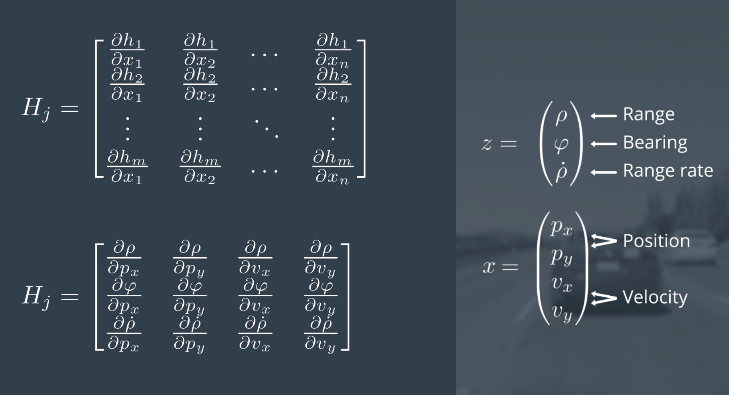
\includegraphics[width=1\linewidth, height=5cm]{jacobian_p1}
   \caption{General Jacobian}
   \label{fig:jacobian_p1} 
\end{subfigure}

\begin{subfigure}[b]{0.9\textwidth}
   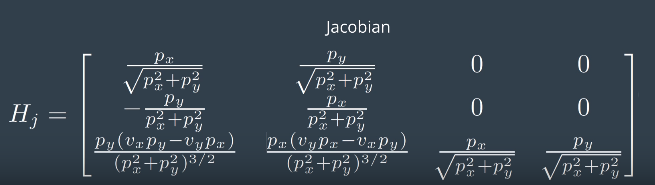
\includegraphics[width=1\linewidth, height=3cm]{jacobian_p2}
   \caption{Jacobian for this case}
   \label{fig:jacobian_p2}
\end{subfigure}

\caption[]{}
\end{figure}






\section{Extended Kalman Filter Algorithm Generalization}%
\label{sec:ekf_generalization}



What I changed is that I used my nonlinear function f(x) to predict the state and h(x) to compute the measurement error.


Additionaly, the state transition matrix F, and the measurement matrix H, are replaced by corresponding Jacobians $F_j$ and $H_j$. I have to recompute the Jacobians every time. 

So, for the EKF I first linearise the nonlinear prediction and measurement functions, and then I just I just use the same Kalman Filter mechanism.



\subsection{Extended Kalman Filter Equations}%
\label{sub:extended_kalman_filter_equations}



Although the mathematical proof is somewhat complex, it turns out that the Kalman filter equations and extended Kalman filter equations are very similar. The main differences are:

\begin{itemize}
	\item The $F$ matrix will be replaced by $F_j$ when calculating $P'$
	\item The $H$ matrix in the Kalman filter will be replaced by the Jacobian matrix $H_j$ when calculating $S$, $K$, and $P$. 
	\item to calculate $x'$, the prediction update function $f$, is used instead of the $F$ matrix.
	\item to calculate $y$, the $h$ function is used instead of the $H$ matrix.
\end{itemize}


For this project, however, we do not need to use the $f$ function of $F_j$. If we had been using a non-linear model in the prediction step, we would need to replace the $F$ matrix with its Jacobian, $F_j$. However, we are using a linear model for the prediction step. So, for the prediction step, we can still use the regular Kalman filter equations and the $F$ matrix rather than the extended Kalamn filter equations.


The measurement update for lidar will also use the regular Kalman filter equations, since lidar uses linear equations. Only the measurement update for the radar sensor will use the extended Kalman filter equations.



\textbf{One important point to reiterate is that the equation $y = z - Hx'$ for the Kalman filter does not become $y = z - H_j x$ for the extended Kalman filter. Instead, for extended Kalman filters, we'll use the h function directly to map predicted locations $x'$ from Cartesian to polar coordinates.}



\begin{figure}[htpb!]
	\centering
	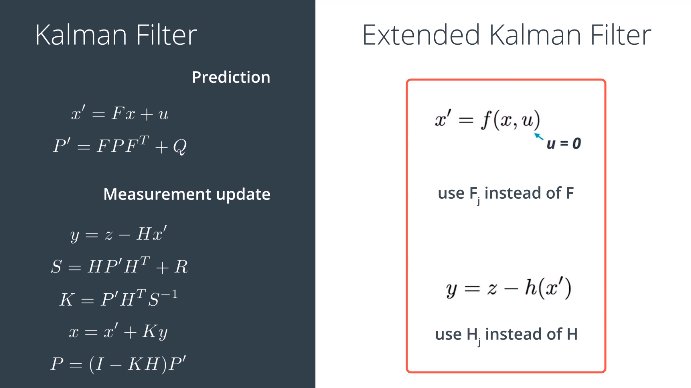
\includegraphics[width=0.8\linewidth]{EKF_alforithm_generalization}
	\caption{EKF algorithm Generalization}
	\label{fig:EKF_alforithm_generalization}
\end{figure}


\subsection{Clarification of u = 0}%
\label{sub:clarification_of_u_0_}



In the above image, the prediction equation is written as $x' = Fx + u$ and $x' = f(x,u)$. Previously the equation was written $x' = Fx + \nu$.  It is just a question of notation where $\nu$ is the greek letter "nu" and "u" is used in the code examples. Remember that $\nu$ is represented by a gaussian distribution with mean zero. The equation $x' = Fx + u$ or the equivalent equation $x' = Fx + \nu$ calculates the mean value of the state variable $x$; hence we set u = 0. The uncertainty in the gaussian distribution shows up in the $Q$ matrix.




\subsection{More Details About Calculations with Radar vs Lidar}%
\label{sub:more_details_about_calculations_with_radar_vs_lidar}


In the radar update step, the Jacobian matrix $H_j$ is used to calculate S, K and P. To calculate y, we use the equations that map the predicted location $x'$ from Cartesian coordinates to polar coordinates:


\[
	h\left(x^{\prime}\right)=\left(\begin{array}{c}{\rho} \\ {\varphi} \\ {\dot{\rho}}\end{array}\right)= \left(\begin{array}{c}{\sqrt{p_{x}^{\prime 2}+p^{\prime2}_{y}}} \\ 
	{\operatorname{arctan}\left(p_{y}^{\prime} / p_{x}^{\prime}\right)} \\ 
{\frac{p_{x}^{\prime} v_{x}^{\prime}+p_{y} v_{y}^{\prime}}{\sqrt{p_{x}^{\prime2}+p_{y}^{\prime2}}}}\end{array}\right)
.\] 




The predicted measurement vector $x'$ is a vector containing values in the form $[p_x, p_y, \nu_x, \nu_y]$. The radar sensor will output values in polar coordinates:

\[
\left(\begin{array}{l}{\rho} \\ {\phi} \\ {\dot{\rho}}\end{array}\right)
.\] 

In order to calculate $y$ for the radar sensor, we need to convert $x'$ to polar coordinates. In other words, the function $h(x)$ maps values from Cartesian coordinates to polar coordinates. So the equation for radar becomes $y = z_{radar} - h(x')$



One other important point when calculating $y$ with radar sensor data: the second value in the polar coordinate vector is the angle $\phi$. You'll need to make sure to normalize $\phi$ in the $y$ vector so that its angle is between $-\pi$ and $pi$; in other words, add or subtract $2\pi$ from $\phi$ until is between $-\pi$ and $\pi$.

To summarize:

\begin{itemize}
	\item For measurement updates with lidar, we can use the $H$ matrix for calculating $y$, $S$, $K$ and $P$.
	\item For radar, $H_j$ is used to calculate $S$, $K$, and $P$.
\end{itemize}















\section{Questions}%
\label{sec:questions}


\textbf{1. Why do we not use the process noise in the state prediction function, even though the state transition equation has one? In other words, why does the code set $u << 0,0$ for the equation $x = F * x + u$}


Because the noise mean is zero.
The noise covariance $Q$ is added to the state covariance prediction so that the state uncertainty always increases through the process noise. 


\textbf{2. Suppose you have a pedestrian state X. I want you to compare two scenarios: in the first predict the state 0.1s into the future and in the second 5s into the future. Which of these two scenarios leads to a higher uncertainty? In answering this, consider whether or not random noise has an increasing effect with increasing gaps between prediction times.}

Right! Here's another way of thinking about it: if you split the 5s time difference into several intermediate predictions with a difference of 0.1s, then compared to the first case, you will predict the same state many more times without receiving any feedback about the object's new position. Thus, the uncertainty increases.



\textbf{3. Let's say we use our linear motion model with fixed time increments, but the pedestrian is randomly changing her velocity (accelerating), sometimes speeding up, slowing down or changing direction. However, the overall mean change is zero. This introduces a noise in the tracking process - what kind of noise is it?}

It's not measurement noise because is during the prediction step that we apply our belief that the pedestrian is moving with constant velocity. So, the prediction equation treats the pedestrain's velocity as constant. As such, a randomly accelerating pedestrian creates a process noise.


\textbf{4. Compared to Kalman Filters, how would the Extended Kalman Filter result differ when the prediction function and measurement function are both linear?}

If $f$ and $h$ are linear functions, then the EKF generates exactly the same result as the standard Kalman Filter. Actually, if $f$ and $h$ are linear then the EKF $F_j$ turns into $F$ and $H_j$ into $h$.
In our case we have a linear motion model, but a nonlinear measurement model when we use radar observations. So, we have to compute the Jacobian only for the measurement function.



\section{Additional Resources}%
\label{sec:additional_resources}

\subsection{Tracking Multiple Objects and Sensor Fusion}%
\label{sub:tracking_multiple_objects_and_sensor_fusion}


The below papers and resources concern tracking multiple objects, using Kalman Filters as well as other techniques!  \\

\href{https://arxiv.org/pdf/1802.08755.pdf}{No Blind Spots: Full-Surround Multi-Object Tracking for Autonomous Vehicles using Cameras \& LiDARs by A. Rangesh and M. Trivedi}

Abstract: Online multi-object tracking (MOT) is extremely important for high-level spatial reasoning and path planning for autonomous and highly-automated vehicles. In this paper, we present a modular framework for tracking multiple objects (vehicles), capable of accepting object proposals from different sensor modalities (vision and range) and a variable number of sensors, to produce continuous object tracks. [...] We demonstrate that our framework is well-suited to track objects through entire maneuvers around the ego-vehicle, some of which take more than a few minutes to complete. We also leverage the modularity of our approach by comparing the effects of including/excluding different sensors, changing the total number of sensors, and the quality of object proposals on the final tracking result. \\



\href{https://hal.archives-ouvertes.fr/hal-01241846/document}{Multiple Sensor Fusion and Classification for Moving Object Detection and Tracking by R.O. Chavez-Garcia and O. Aycard}

Abstract: [...] We believe that by including the objects classification from multiple sensors detections as a key component of the object’s representation and the perception process, we can improve the perceived model of the environment. First, we define a composite object representation to include class information in the core object’s description. Second, we propose a complete perception fusion architecture based on the Evidential framework to solve the Detection and Tracking of Moving Objects (DATMO) problem by integrating the composite representation and uncertainty management. Finally, we integrate our fusion approach in a real-time application inside a vehicle demonstrator from the interactIVe IP European project which includes three main sensors: radar, lidar and camera. [...] \\


\subsection{Stereo Cameras}%
\label{sub:stereo_cameras}

The below papers cover various methods of using stereo camera set-ups for object detection and tracking. \\


\href{http://www.cse.cuhk.edu.hk/~khwong/J2008_IEEE_TIM_Stereo%20Kalman%20.pdf}{Robust 3-D Motion Tracking from Stereo Images: A Model-less Method by Y.K. Yu, et. al.}

Abstract: Traditional vision-based 3-D motion estimation algorithms require given or calculated 3-D models while the motion is being tracked. We propose a high-speed extended Kalman filter-based approach that recovers camera position and orientation from stereo image sequences without prior knowledge as well as the procedure for the reconstruction of 3-D structures. [...] The proposed method has been applied to recover the motion from stereo image sequences taken by a robot and a hand-held stereo rig. The results are accurate compared to the ground truths. It is shown in the experiment that our algorithm is not susceptible to outlying point features with the application of a validation gate \\



\href{http://hss.ulb.uni-bonn.de/2010/2356/2356.pdf}{Vehicle Tracking and Motion Estimation Based on Stereo Vision Sequences by A. Barth (long read)}

Abstract: In this dissertation, a novel approach for estimating trajectories of road vehicles such as cars, vans, or motorbikes, based on stereo image sequences is presented. Moving objects are detected and reliably tracked in real-time from within a moving car. [...] The focus of this contribution is on oncoming traffic, while most existing work in the literature addresses tracking the lead vehicle. The overall approach is generic and scalable to a variety of traffic scenes including inner city, country road, and highway scenarios. [...] The key idea is to derive these parameters from a set of tracked 3D points on the object’s surface, which are registered to a time-consistent object coordinate system, by means of an extended Kalman filter. Combining the rigid 3D point cloud model with the dynamic model of a vehicle is one main contribution of this thesis. [...] The experimental results show the proposed system is able to accurately estimate the object pose and motion parameters in a variety of challenging situations, including night scenes, quick turn maneuvers, and partial occlusions.\\



\subsection{Deep Learning-based approaches}%
\label{sub:deep_learning_based_approaches}


\href{http://openaccess.thecvf.com/content_cvpr_2018/papers/Luo_Fast_and_Furious_CVPR_2018_paper.pdf}{Fast and Furious: Real Time End-to-End 3D Detection, Tracking and Motion Forecasting with a Single Convolutional Net by W. Luo, et. al.}

Abstract: In this paper we propose a novel deep neural network that is able to jointly reason about 3D detection, tracking and motion forecasting given data captured by a 3D sensor. By jointly reasoning about these tasks, our holistic approach is more robust to occlusion as well as sparse data at range. Our approach performs 3D convolutions across space and time over a bird’s eye view representation of the 3D world, which is very efficient in terms of both memory and computation. Our experiments on a new very large scale dataset captured in several north american cities, show that we can outperform the state-of-the-art by a large margin. Importantly, by sharing computation we can perform all tasks in as little as 30 ms. \\



\href{https://arxiv.org/abs/1711.06396}{VoxelNet: End-to-End Learning for Point Cloud Based 3D Object Detection by Y. Zhou and O. Tuzel}


Abstract: Accurate detection of objects in 3D point clouds is a central problem in many applications, such as autonomous navigation, housekeeping robots, and augmented/virtual reality. To interface a highly sparse LiDAR point cloud with a region proposal network (RPN), most existing efforts have focused on hand-crafted feature representations, for example, a bird's eye view projection. In this work, we remove the need of manual feature engineering for 3D point clouds and propose VoxelNet, a generic 3D detection network that unifies feature extraction and bounding box prediction into a single stage, end-to-end trainable deep network. [...] Experiments on the KITTI car detection benchmark show that VoxelNet outperforms the state-of-the-art LiDAR based 3D detection methods by a large margin. Furthermore, our network learns an effective discriminative representation of objects with various geometries, leading to encouraging results in 3D detection of pedestrians and cyclists, based on only LiDAR.\\


\subsection{Papers on Tracking Multiple objects and Sensor Fusion}%
\label{sec:other_papers_on_tracking_multiple_objects_and_sensor_fusion}


\href{http://www.ejaet.com/PDF/2-2/EJAET-2-2-34-39.pdf}{Multiple Object Tracking using Kalman Filter and Optical Flow by S. Shantaiya, et. al.} \\

\href{https://pdfs.semanticscholar.org/f5a2/bf3df3126d2923a617b977ec2b4e1c829a08.pdf}{Kalman Filter Based Multiple Objects Detection-Tracking Algorithm Robust to Occlusion by J-M Jeong, et. al.} \\

\href{https://arxiv.org/pdf/1802.01235.pdf}{Tracking Multiple Moving Objects Using Unscented Kalman Filtering Techniques by X. Chen, et. al.} \\

\href{https://velodynelidar.com/lidar/hdlpressroom/pdf/Articles/LIDAR-based%203D%20Object%20Perception.pdf}{LIDAR-based 3D Object Perception by M. Himmelsbach, et. al} \\

\href{https://www.researchgate.net/publication/309503024_Fast_multiple_objects_detection_and_tracking_fusing_color_camera_and_3D_LIDAR_for_intelligent_vehicles}{Fast multiple objects detection and tracking fusing color camera and 3D LIDAR for intelligent vehicles by S. Hwang, et. al.} \\

\href{https://repository.tudelft.nl/islandora/object/uuid%3Af536b829-42ae-41d5-968d-13bbaa4ec736}{3D-LIDAR Multi Object Tracking for Autonomous Driving by A.S. Rachman (long read)} 







\end{document}
